\documentclass[a4paper,oneside,article,10pt]{memoir}
\usepackage{graphicx}
\usepackage{mathtools}
\usepackage{wasysym}
\usepackage{amsmath}
\usepackage{amsfonts}
\usepackage{xparse}
\usepackage{graphicx}
\usepackage{subfig}
\numberwithin{equation}{section}
\usepackage{authblk}
\usepackage[utf8x]{inputenc}
\usepackage{wasysym}
\usepackage[colorlinks=true]{hyperref}
\usepackage{slashed}
\usepackage{amssymb}

\usepackage{cleveref}
\usepackage{listings}
%\usepackage{minted}
\usepackage{microtype}
\usepackage[font={small,it}]{caption}
\setlength{\oddsidemargin}{-0in}
\setlength{\textwidth}{6.2in}




\title{\Huge Natural logarithm (integral representation)}
\author{Alexander S. Madsen \thanks{e-mail: asm.arbejde@gmail.com}\\
Institute for Physics og Astronomi, Aarhus Universitet, Denmark}


\date{\today} %Dato. Kan evt. ændres, hvis I ikke har lavet rapporten idag.

\begin{document}
\maketitle


\chapter{Introduction}
In the following we are asked to implement a function that calculates the natural logarithm of a real positive number $x$ using the integral representation
\begin{equation}
  \ln(x) = \int_1^x \frac{1}{t} \,dt\label{eq:ln_int}
\end{equation}
The integration is to be carried out using a suitable GSL integration routine. Furthermore, to improve computational efficiency, the integration interval must be \textit{reduced} before the routine is called such that $1\leq x < 2$ for an arbitrary positive number $x$. This is to be done using the formulas
\begin{equation}
  \ln(x) = -\ln\left(\frac{1}{x}\right)\, , \, \ln(x)=\ln(2)+\ln\left(\frac{x}{2}\right)
\end{equation}
Finally the acquired results must be compared to a with $\ln(x)$ function from the $<\text{math.h}>$ library or from GSL.

\chapter{Implementation}
 A separate $c$-file called \textit{log\_int.c} is build containing a numerical implementation of \cref{eq:ln_int}, compliant with the specification of the GSL library $\text{h}$, as well as a function executing the GSL integration routine itself. 
 Specifically the function takes a \textit{double} $x$ corresponding to the upper integration limit in \cref{eq:ln_int} and returns the \textit{double result}. The function automatically allocates and frees the workspace needed for the particular GSL integration routine which for this problem is set to be gsl\_integration\_qags. 
 The "projection" of the positive variable $x$ onto the interval $1\leq x < 2$ is implemented by nesting the function within itself using the following if-statement sequence 
 \begin{lstlisting}
 		if(x < 1){return -log_int(1.0/x, calls);}
 		if(x >= 2){return log(2.0) + log_int(x/2.0, calls);}
 \end{lstlisting}
This results in a recursion in which the function continuously calls itself until the condition $1\leq x < 2$ is realized at which point the GSL integration routine is carried out.
The program is run from the c-file main.c by calling log\_int in a for loop. Specifically the function is evaluated from $0.1$ to $10$ using a step size of $\Delta x = 0.1$. 


\chapter{Results and Conclusion}
Figure shows a plot of the data points contained from the datafile \textit{out.txt} created when the script is run.
\begin{figure}[h!]
	\centering
	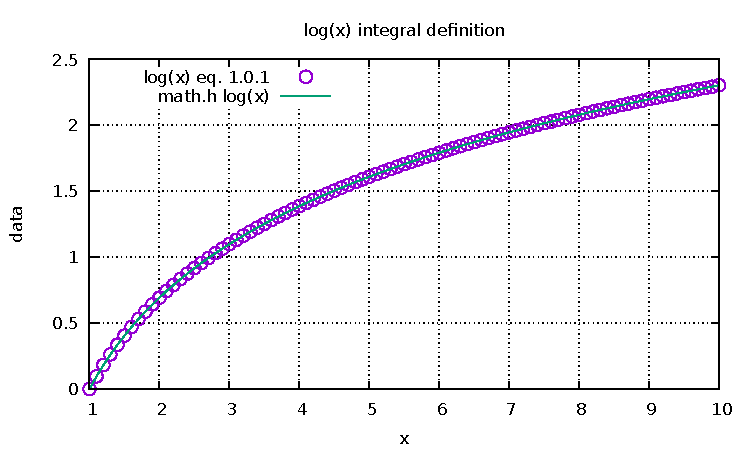
\includegraphics[]{figure.pdf}
	\caption{Result from running the main.c script. The figure shows the \cref{eq:ln_int} from $x=[1,10]$ and overlayed of the $\ln(x)$ from the math.h library}
	\label{fig.log}
\end{figure}
It is evident from \cref{fig.log} that the routine produces sensible values of $\ln(x)$. Hence we can conclude that \cref{eq:ln_int}, with the required reduction of the integration, is meaningful and computationally efficient way to calculate $\ln(x)$ 





















\end{document}
